
\section{Einleitung}
\label{sec:intro}

Das \textit{multi-car multi-color paint shop} Problem beschreibt die Herausforderung der optimalen Zuordnung von Farben zu Fahrzeugen in einer Produktionslinie. Da die Reihenfolge der Fahrzeuge arbiträr, und jeder Farbwechsel mit Aufwand verbunden ist, liegt ein besonderes Interesse darin, die  Zuordnung der Farben zu den Fahrzeugkonfigurationen so zu optimieren, dass die Anzahl der Farbwechsel minimiert wird. Formal lässt sich dieses Problem wie folgt definieren:\\

\noindent Seien\\
\begin{tabular}{lp{0.6\linewidth}}

eine Menge $K=\{\omega_0, ..., \omega_l\}$&verschiedene Fahrzeugkonfigurationen\\
&Beispiel: \{Golf, Polo\}\\
\\
eine Menge $F=\{\varphi_0, ..., \varphi_m\}$&verschiedene Fahrzeugfarben,\\
&Beispiel: \{rot, blau\}\\
\\
eine Menge $D\subseteq K\times F$&Tupel aus Fahrzeugkonfigurationen und Farben,\\
&Beispiel: \{(Golf, rot),(Golf, blau),(Polo, rot)\}\\
\\
eine Funktion $\sigma:D\to \mathbb{N}$&Häufigkeit der Konfigurations-Farb-Kombinationen,\\
&Beispiel: $\sigma(Golf,rot) = 2$\\
\\
eine Variable $N$&Anzahl von Konfigurationen in der Produktionslinie,\\
&Beispiel: 6\\
\\
eine Variable $X_{n,\varphi}$&Konfiguration an Stelle n hat die Farbe $\varphi$ \\
&Beispiel: $X_{1,rot} = 1$; $X_{1,blau} = 0$\\
\\
ein Vektor $\pi:\{1,...,N\}\to K$&die Produktionslinie,\\
&Beispiel: [Golf, Polo, Golf, Golf, Golf, Golf]\\
\\
ein Vektor $\gamma:\{1,...,N\}\to F$&die Zuordnung der Farben zu den Konfigurationen in der Produktionslinie,\\
&Beispiel: [rot, rot, blau, blau, blau, rot]\\
\\
eine Funktion $cost:\mathbb{F}(\{1,...,N\}, F) \to \mathbb{N}$&Anzahl der Farbwechsel,\\
\\
\end{tabular}

\noindent Gesucht: $\arg\min {cost(\gamma)}$\\
\\
\noindent Bedingungen

Jede Position in der Produktionslinie hat \underline{genau} eine Farbe 
\begin{equation}
\displaystyle\sum_{n\leq N}\left(\sum_{\varphi\in F} X_{n,\varphi} - 1\right)^2
\end{equation}

Jede Konfigurations-Farb-Kombination kommt so häufig vor wie angegeben 
\begin{equation}
\displaystyle\sum_{\omega,\varphi\in D}\left ({\sum_{n,\pi(n)=\omega} X_{n,\varphi}} - \sigma(\omega,\varphi)\right )^2
\end{equation}

Die Anzahl der Farbwechsel ist minimal
\begin{equation}
\displaystyle\sum_{n=1}^{N-1} \sum_{\varphi\in F} (X_{n,\varphi} -X_{n+1,\varphi})^2
\end{equation}

\section{Grundlagen}
\label{sec:basics}

\section{Verwandte Arbeiten}
\label{sec:related}


\section{Konzept}
\label{sec:concept}

\begin{figure}[h]
 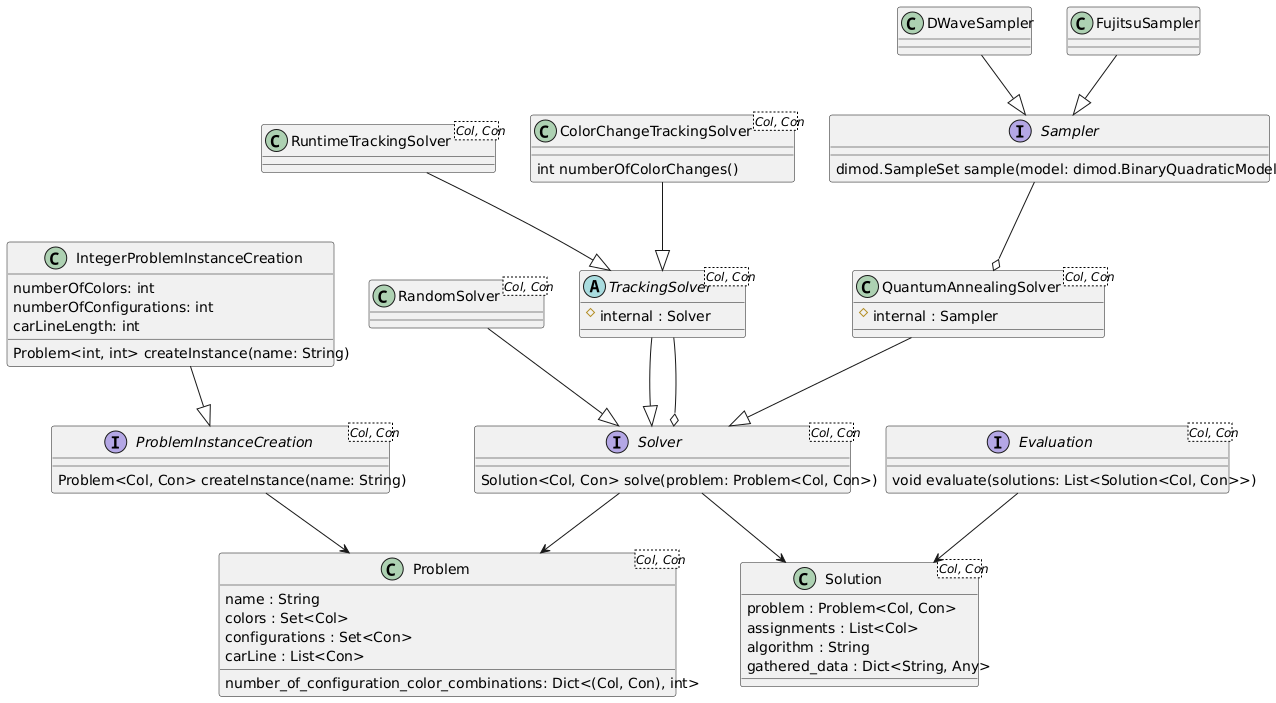
\includegraphics[width=\linewidth]{./images/problem.png}
 \caption{Problem UML}
 \label{fig:uml1}
\end{figure}

\subsection{QUBO-Formulierung}
\label{subsec:qubo}


\subsection{Trainingsmethode}
\label{subsec:training}


\section{Evaluation}
\label{sec:evaluation}


\subsection{Annealing}
\label{subsec:annealing}


\subsection{Gate Model}
\label{subsec:qgm}


\section{Fazit}
\label{sec:conclusion}


